\chapter{Metodo di Jacobi}

\subsection*{Introduzione}

Consideriamo il sistema lineare

\begin{equation}
	A \boldsymbol{\phi} = \boldsymbol{s}
\end{equation}

dove $A \in \mathbb{R}^{n \times n}$ è una matrice assegnata, $\boldsymbol{\phi}$ il vettore incognito e $\boldsymbol{s}$ il termine noto.

Il metodo di Jacobi si basa sulla decomposizione della matrice $A$ nella forma

\begin{equation}
	A = D - E
\end{equation}

dove: $D$ è la matrice diagonale contenente gli elementi diagonali di $A$ mentre $E$ contiene l'opposto degli elementi fuori diagonale di $A$.

Sostituendo nella relazione iniziale si ottiene:

\begin{equation}
	D \boldsymbol{\phi} = E \boldsymbol{\phi} + \boldsymbol{s}
\end{equation}

Assumendo che $D$ sia invertibile (cioè $a_{ii} \neq 0$ per ogni $i$), si può scrivere

\begin{equation}
	\boldsymbol{\phi} = D^{-1} E \boldsymbol{\phi} + D^{-1} \boldsymbol{s}
\end{equation}

Introducendo le definizioni

\begin{equation}
	H = D^{-1} E, \qquad \boldsymbol{q} = D^{-1} \boldsymbol{s}
\end{equation}

il sistema assume la forma

\begin{equation}
	\boldsymbol{\phi} = H \boldsymbol{\phi} + \boldsymbol{q}
\end{equation}

\subsection*{Struttura della matrice di iterazione}

Dalla struttura di $D$ ed $E$ si ottiene che la matrice $H$ ha forma

\begin{equation}
	H =
	\begin{pmatrix}
		0 & -\frac{a_{12}}{a_{11}} & -\frac{a_{13}}{a_{11}} & \cdots & -\frac{a_{1n}}{a_{11}} \\
		-\frac{a_{21}}{a_{22}} & 0 & -\frac{a_{23}}{a_{22}} & \cdots & -\frac{a_{2n}}{a_{22}} \\
		\vdots & \vdots & \vdots & & \vdots \\
		-\frac{a_{n1}}{a_{nn}} & -\frac{a_{n2}}{a_{nn}} & -\frac{a_{n3}}{a_{nn}} & \cdots & 0
	\end{pmatrix}
\end{equation}

Gli elementi diagonali sono nulli.

Se la matrice $A$ è diagonalmente dominante, vale

\begin{equation}
	\sum_{j=1}^{n} |h_{ij}| < 1 \quad \forall i
\end{equation}

da cui segue

\begin{equation}
	\|H\|_\infty < 1 \quad \Rightarrow \quad \rho(H) < 1
\end{equation}

Quindi la matrice $H$ è convergente.

\subsection*{Procedimento iterativo}

Si introduce il processo iterativo

\begin{equation}
	\boldsymbol{\phi}^{(m+1)} = H \boldsymbol{\phi}^{(m)} + \boldsymbol{q}
\end{equation}

con condizione iniziale

\begin{equation}
	\boldsymbol{\phi}^{(1)} = \boldsymbol{q}
\end{equation}

Esplicitando le iterazioni:

\begin{align}
	\boldsymbol{\phi}^{(2)} &= H \boldsymbol{\phi}^{(1)} + \boldsymbol{q} = H \boldsymbol{q} + \boldsymbol{q} \\
	\boldsymbol{\phi}^{(3)} &= H^2 \boldsymbol{q} + H \boldsymbol{q} + \boldsymbol{q} \\
	\vdots \\
	\boldsymbol{\phi}^{(m+1)} &= H^m \boldsymbol{q} + H^{m-1} \boldsymbol{q} + \cdots + \boldsymbol{q}
\end{align}

\subsection*{Convergenza del metodo}

Moltiplicando per $(I - H)$ si ottiene

\begin{equation}
	(I - H)\boldsymbol{\phi}^{(m+1)} = (I - H^{m+1}) \boldsymbol{q}
\end{equation}

e quindi

\begin{equation}
	\boldsymbol{\phi}^{(m+1)} = (I - H)^{-1} (I - H^{m+1}) \boldsymbol{q}
\end{equation}

Passando al limite

\begin{equation}
	\lim_{m \to \infty} \boldsymbol{\phi}^{(m+1)} = (I - H)^{-1} \boldsymbol{q}
\end{equation}

D'altra parte, la soluzione esatta soddisfa

\begin{equation}
	\boldsymbol{\phi} = H \boldsymbol{\phi} + \boldsymbol{q}
\end{equation}

da cui

\begin{equation}
	(I - H)\boldsymbol{\phi} = \boldsymbol{q}
	\quad \Rightarrow \quad
	\boldsymbol{\phi} = (I - H)^{-1} \boldsymbol{q}
\end{equation}

Quindi

\begin{equation}
	\lim_{m \to \infty} \boldsymbol{\phi}^{(m)} = \boldsymbol{\phi}
\end{equation}

\subsection*{Studio della convergenza tramite autovalori}

Sia $H$ simmetrica. Allora esiste una matrice ortogonale $U$ tale che

\begin{equation}
	U^T H U = \Lambda
\end{equation}

dove $\Lambda = \text{diag}(\lambda_1, \dots, \lambda_n)$.

Segue che

\begin{equation}
	H \boldsymbol{u}_j = \lambda_j \boldsymbol{u}_j
\end{equation}

Gli autovettori formano una base ortonormale.

\subsection{Errore}

Definiamo l'errore

\begin{equation}
	\boldsymbol{\varepsilon}^{(m)} = \boldsymbol{\phi}^{(m)} - \boldsymbol{\phi}
\end{equation}

Si ha

\begin{equation}
	\boldsymbol{\varepsilon}^{(m)} = H^m \boldsymbol{\varepsilon}^{(0)}
\end{equation}

Sviluppando sull'autobase:

\begin{equation}
	\boldsymbol{\varepsilon}^{(0)} = \sum_{h=1}^n c_h^{(0)} \boldsymbol{\phi}_h
\end{equation}

\begin{equation}
	\boldsymbol{\varepsilon}^{(m)} = \sum_{h=1}^n c_h^{(0)} \lambda_h^m \boldsymbol{\phi}_h
\end{equation}

La convergenza avviene se e solo se

\begin{equation}
	|\lambda_h| < 1 \quad \forall h
\end{equation}

cioè

\begin{equation}
	\rho(H) < 1
\end{equation}

\subsection*{Condizioni di convergenza}

Una condizione sufficiente per la convergenza è che la matrice $A$ sia strettamente diagonalmente dominante:

\begin{equation}
	|a_{ii}| > \sum_{j \neq i} |a_{ij}|
\end{equation}

Oppure irriducibilmente diagonalmente dominante:

\begin{equation}
	|a_{ii}| \ge \sum_{j \neq i} |a_{ij}|
\end{equation}

con almeno una riga per cui la disuguaglianza è stretta.

\subsection*{Definizione di irriducibilità}

Una matrice è riducibile se esiste una matrice di permutazione $P$ tale che

\begin{equation}
	P A P^T =
	\begin{pmatrix}
		\hat{A}_{11} & \hat{A}_{12} & \cdots \\
		0 & \hat{A}_{22} & \cdots \\
		\vdots & \vdots & \ddots
	\end{pmatrix}
\end{equation}

Se ciò non è possibile, la matrice è detta irriducibile.

Una matrice è irriducibile se e solo se il suo grafo orientato è fortemente connesso.

\begin{figure}[H]
	\label{connected}
	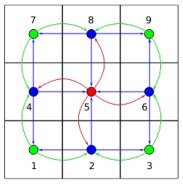
\includegraphics[width=6cm]{img/graph-connected.png}
	\caption{catzo e palle}
\end{figure}

\begin{figure}[H]
	\label{not connected}
	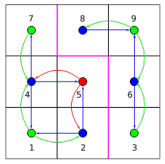
\includegraphics[width=6cm]{img/graph-not-connected.png}
	\caption{catzo e palle}
\end{figure}

\subsection*{Schema esplicito del metodo di Jacobi}

Il sistema

\begin{equation}
	\sum_{j=1}^n a_{ij} \phi_j = b_i
\end{equation}

viene risolto iterativamente come

\begin{equation}
	\phi_i^{(m+1)} =
	\frac{1}{a_{ii}}
	\left(
	b_i - \sum_{j \neq i} a_{ij} \phi_j^{(m)}
	\right)
\end{equation}

\subsection*{Implementazione per equazione di diffusione}

Nel caso bidimensionale:

\begin{equation}
	- \frac{D}{h_x^2} (\phi_{i+1,j} - 2\phi_{i,j} + \phi_{i-1,j})
	- \frac{D}{h_y^2} (\phi_{i,j+1} - 2\phi_{i,j} + \phi_{i,j-1})
	+ \Sigma_a \phi_{i,j} = Q_{i,j}
\end{equation}

Definendo

\begin{align}
	W_{i,j} = E_{i,j} &= \frac{D/h_x^2}{\Sigma_a + 2D/h_x^2 + 2D/h_y^2} \\
	S_{i,j} = N_{i,j} &= \frac{D/h_y^2}{\Sigma_a + 2D/h_x^2 + 2D/h_y^2} \\
	q_{i,j} &= \frac{Q_{i,j}}{\Sigma_a + 2D/h_x^2 + 2D/h_y^2}
\end{align}

lo schema diventa

\begin{equation}
	\phi_{i,j}^{(m+1)} =
	W_{i,j}\phi_{i-1,j}^{(m)} +
	E_{i,j}\phi_{i+1,j}^{(m)} +
	S_{i,j}\phi_{i,j-1}^{(m)} +
	N_{i,j}\phi_{i,j+1}^{(m)} +
	q_{i,j}
\end{equation}

\subsection*{Velocità di convergenza}

L'errore si comporta come

\begin{equation}
	\|\varepsilon^{(m)}\| \approx C \rho(H)^m
\end{equation}

e vale

\begin{equation}
	\lim_{m \to \infty}
	\frac{\|\varepsilon^{(m+1)}\|}{\|\varepsilon^{(m)}\|}
	= \rho(H)
\end{equation}

Il tasso asintotico di convergenza è

\begin{equation}
	R_\infty(H) = -\ln \rho(H)
\end{equation}

\subsection*{Numero di iterazioni}

Per ridurre l'errore di un fattore $\sigma$:

\begin{equation}
	\rho(H)^n < \sigma
\end{equation}

da cui

\begin{equation}
	n > \frac{\ln \sigma}{\ln \rho(H)}
	= -\frac{\ln \sigma}{R_\infty(H)}
\end{equation}

\subsection*{Osservazioni finali}

Per avere una convergenza veloce è necessario che

\begin{equation}
	\rho(H) \ll 1
\end{equation}

Si osserva che:

\begin{itemize}
	\item se $\Sigma_a \to 0$, la dominanza diagonale diminuisce e $\rho(H) \to 1$;
	\item raffinando la griglia ($h_x, h_y \to 0$), $\rho(H) \to 1$;
\end{itemize}

quindi una maggiore risoluzione spaziale comporta una convergenza più lenta.

\begin{figure}[H]
	\label{jacobi}
	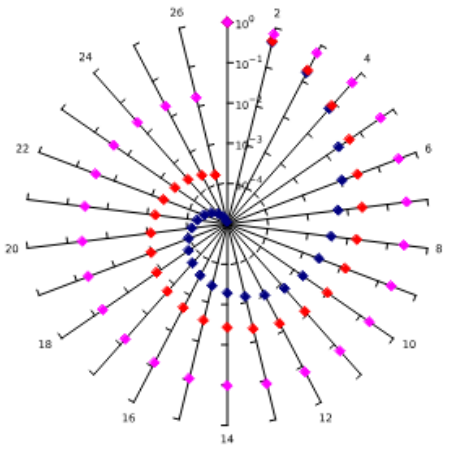
\includegraphics[width=6cm]{img/Jacobi.png}
	\caption{catzo e palle}
\end{figure}